\documentclass[11pt,paper=a4,answers]{exam}
\usepackage{graphicx,lastpage}
\usepackage{upgreek}
\usepackage{censor}
\usepackage{tabularx}
\usepackage{xcolor}
\usepackage{amsmath}
\usepackage{cleveref}
\usepackage{tabularx,pbox}
\usepackage[nopar]{lipsum}
\usepackage{longtable}
\usepackage{multirow}
\usepackage[inline]{enumitem}
\usepackage{float}
\usepackage{pdfrender}
\usepackage{pgfplots}  
\pgfplotsset{width=7cm,compat=1.7}  
\setlength{\parindent}{0pt}
	\definecolor{blue(pigment)}{rgb}{0.2, 0.2, 0.6}
\flushbottom
\usepackage[normalem]{ulem}
%\renewcommand\ULthickness{2pt}   %%---> For changing thickness of underline
%\setlength\ULdepth{1.5ex}%\maxdimen ---> For changing depth of underline
%\renewcommand{\baselinestretch}{1}
%\pagestyle{empty}
\pagestyle{headandfoot}

\newcommand{\continuedmessage}{%
%\ifcontinuation{\footnotesize Question \ContinuedQuestion\ continues\ldots}{}%
 }
%\runningheader{\footnotesize Mathematics}
%{\footnotesize Mathematics --- Differential Geometry}
%{\footnotesize Page \thepage\ of \numpages}
%\footrule
\begin{document}
	\setlength{\tabcolsep}{10pt}
\renewcommand{\arraystretch}{1.5}
Hall Ticket No 
\begin{tabular}{|c| c| c| c| c| c|c| c| c| c|} \hline
	& & &&&&&&&\\ [0.5ex]\hline
\end{tabular}
\hfill Question Paper Code: AAEC35
\vspace{5pt}\hrule
\vspace{5pt}
\crefname{figure}{figure}{figures}
\crefname{question}{question}{questions}
%==============================================================

\begin{minipage}{0.15\linewidth}%
	\flushleft
	
\includegraphics[width=0.85\textwidth]{iare.png}\end{minipage}
%% \thispagestyle{empty}
\begin{minipage}[r]{0.85\textwidth}%
	\noindent
	\begin{center}	
	\textcolor{blue}{\Large \bfseries INSTITUTE OF AERONAUTICAL ENGINEERING}\\
	%\hspace*{5.2cm} 
	\textcolor{blue}{\Large (Autonomous)} \\
	%\hspace*{4.7cm}
	\small Dundigal, Hyderabad - 500 043 \\  [3pt] 
	%\hspace*{4.2cm}
	\framebox[1.2\width]{MODEL QUESTION PAPER-II} \par \vspace{3pt}
	B.Tech VII Semester End Examinations, December–2025 \\ \vspace{3pt}
	Regulations: IARE - UG20 \\\vspace{3pt}
	\textcolor{red}{\large \bfseries AEROSPACE STRUCTURAL DYNAMICS } \\\vspace{3pt}
	\large \bfseries AERONAUTICAL ENGINEERING
\end{center}
\end{minipage}
\vspace{0.5cm}
\par
\noindent
\uline{Time: 3 hour   \hfill  \hfill        Maximum Marks: 70}\\
{\centering
	{\large \bfseries Answer ALL questions in Module I and II  \par
	\large Answer ONE out of two questions in Modules III, IV and V \\[3pt]
	\large All Questions Carry Equal Marks \par 
	\large All parts of the question must be answered in one place only   }
\noindent\hrule
}
\vspace{5pt}
	%%%% Part - A %%%%	
\centering {\textbf{MODULE-I}}\\
\vspace{-0.5cm}
	\begin{questions}
		\question
		\begin{parts}
	\part %1a 
 A damped system has following elements: Mass = 4 kg; k = 1 kN/m; C = 40 N-sec/m. Determine: (a) Damping factor and natural frequency of damped oscillation.  (b) Logarithmic decrement and number of cycles after which the original amplitude is reduced to 20.
	\hfill[BL: Understand| CO: 1|Marks: 7]
			\part%1b	
A mass of 2kg is supported on an isolator having a spring scale of 2940 N/m and viscous damping. If the amplitude of free vibration of the mass falls to one half its original values in 1.5 seconds, determine the damping coefficient of the isolator.
		
			\hfill[BL: Understand| CO: 1|Marks: 7]

	\end{parts}

\centering {\textbf{MODULE-II}}
	\question
	\begin{parts}
\part	%3a	
What is meant by static and dynamic coupling? How can coupling of the equations of motion be eliminated? Derive the governing equations through Lagrange energy approach.

\hfill[BL: Understand| CO: 2|Marks: 7]
\part %3b
Derive the equation of motion of the system shown in figure. Assume that the initial tension ‘T’ in the string is too large and remains constants for small amplitudes. Determine the natural frequencies, the ratio of amplitudes and locate the nodes for each mode of vibrations when m1 = m2= m and l1=l, l2 = 2l, l3 =3l.

\hfill[BL: Understand| CO: 2|Marks: 7]
\begin{figure}[H]
	\centering
	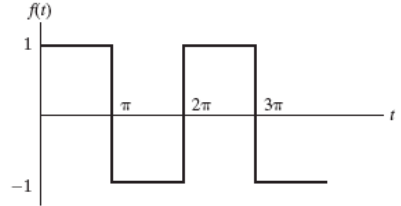
\includegraphics[scale=1.0]{2.png}
	\label{fig:fluiddef}
\end{figure}
\end{parts}

\centering {\textbf{MODULE-III}}\\
\question
\begin{parts}
	\part	%5a	
A seismic instrument is fitted to measure the vibration characteristics of a machine running at 120rpm. If the natural frequency of the instrument is 5Hz and if it shows 0.004cm. Determine the displacement, velocity and acceleration assuming no damping.

	\hfill[BL: Understand| CO: 3|Marks: 7]
	\part	%5b
It is desired to measure maximum acceleration of a machine part, which vibrates violently with a frequency of 700cycles/min. An accelerometer with negligible damping, 0.5 kg mass and 18 KN/m spring constant is attached to it. The total travel of the indicator is found to be 8.2 mm, find the maximum amplitude and maximum acceleration of the part.

	\hfill[BL: Understand| CO: 3|Marks: 7]		 
\end{parts}
\question
 \begin{parts}
\part	%6a 
A vibrometer having a natural frequency of 4 rad/s and $/zeta =0.2$ is attached to a structure performs a harmonic motion. If the difference between the maximum and minimum recorded values is 8mm, find the amplitude of motion of the vibrating structure when its frequency is 40 rad/s.
\hfill[BL: Apply| CO: 3|Marks: 7]
\part	%6b 
Determine the characteristic equation for the system shown in Figure .and solve this equation for the special case when k1= k2= k3 = k and m1 = m2 = m3 = m. Determine if the system has any rigid-body modes.

	\hfill[BL: Apply| CO: 3|Marks: 7]
\begin{figure}[H]
	\centering
	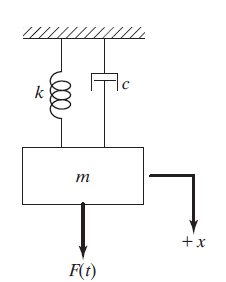
\includegraphics[scale=1.0]{4.png}
	\label{fig:fluiddef}
\end{figure}
\end{parts}
\newpage
\centering {\textbf{MODULE-IV}}
\noindent
\question
 \begin{parts}
	\part  %7a
Explain different types of data acquisition systems with compression to merits and demerits of each other.
  \hfill[BL: Understand| CO: 4|Marks: 7]
	\part  %7b
Machine condition monitoring is very important. Explain thro trending analysis and its interpretation.
	\hfill[BL: Understand| CO: 4|Marks: 7]
\end{parts}
\question\begin{parts}
	\part %8a
Machine condition monitoring is very important. Explain thro trending analysis and its interpretation.
\hfill[BL: Understand| CO: 4|Marks: 7]
	\part  %8a
Name two frequency measuring instruments. Explain any one instrument’s working principle.
 \hfill[BL: Understand| CO: 5|Marks: 7]
\end{parts}
	\centering {\textbf{MODULE-V}}
\question \begin{parts}
	\part      %9a    .
Find the steady state response of a pinned-pinned beam subjected to a harmonic force $f(x,t)=f0\ \sin\left({\omega t}\right) $ applied at x=a as shown in the figure.
  \hfill[BL: Understand| CO: 5|Marks: 7]
\begin{figure}[H]
	\centering
	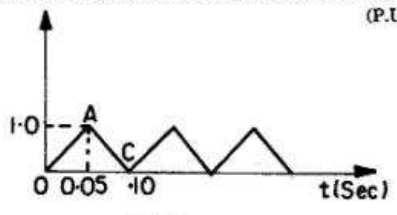
\includegraphics[scale=1.0]{5.png}
	\label{fig:fluiddef}
\end{figure}
	\part  %9b 
A steel wire of 2 mm diameter is fixed between two points located 2 m apart. The tensile force in the wire is 250N. Determine the fundamental natural frequency and the velocity of wave propagation in the wire.
\hfill[BL: Understand| CO: 5|Marks: 7]
\end{parts}
\question 
\begin{parts}
	\part %10a
Determine the natural frequencies of vibration of a uniform beam fixed at x=0 and simply supported at x=l.
\hfill[BL: Understand| CO: 5|Marks: 7]
	\part %10b
Find the value of free-stream velocity u at which the airfoil section (SDOF) shown in Fig becomes unstable
 \hfill[BL: Understand| CO: 5|Marks: 7]
\begin{figure}[H]
	\centering
	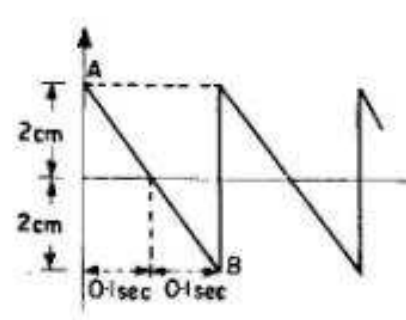
\includegraphics[scale=1.0]{6.png}
	\label{fig:fluiddef}
\end{figure}
\end{parts}
\end{questions}
\hrule
\begin{center}
	\textbf{\text{**END OF EXAMINATION**} }
\end{center}

\flushleft\textbf{\textcolor{blue}{\large COURSE OBJECTIVES:}}
%\vspace{-0.3cm}		

\textbf{The students will try to:}
\vspace{-0.3cm}
\newcolumntype{C}[1]{>{\centering\arraybackslash}p{#1}}
\newcolumntype{R}[1]{>{\raggedright\arraybackslash}p{#1}}
\renewcommand{\arraystretch}{1.2}
\begin{flushleft}	
	\begin{longtable}{|C{1.2cm}|R{15cm}|}
		\hline
		I & Formulate mathematical models of problems in vibrations using Newton’s second law or energy principles.\tabularnewline
		\hline
		II &Determine a complete solution to the modelled mechanical vibration problems.\tabularnewline
		\hline
		III &    design a mechanical system that has desirable vibrational behavior.\tabularnewline
		\hline	
		IV & Assess the underlying assumptions in the aeroelastic analysis of fixed wing and rotary
		wing aerospace vehicles/systems.\tabularnewline
		\hline
	\end{longtable}
\end{flushleft}\vspace{-1.5cm}

\flushleft\textbf{\textcolor{blue}{\large COURSE OUTCOMES:}}\\

%\vspace{-0.3cm}	

\textbf{After successful completion of the course, students should be able to:}\\
\renewcommand{\arraystretch}{1.1}\vspace{-0.75cm}
\begin{flushleft}
	\begin{longtable}{|C{1.5cm}|R{12.5cm}|C{1.5cm}|}
		\hline
		CO 1 &	\textbf{Apply} \textcolor{blue}{ principles of mechanical vibrations such as Newton’s second law, and
			the principle of conservation of energy to the mathematical models  } \textcolor{red}{for obtaining
			their governing equations of motion.}&Apply\tabularnewline
		\hline
		CO 2&	\textbf{Analyze} \textcolor{blue}{   the mathematical modeling of the two degrees of
			freedom systems} \textcolor{red}{ for determining the frequency of the spring-mass system.}&	Apply\tabularnewline
		\hline
		CO 3&	\textbf{Solve} \textcolor{blue}{ the natural frequencies and mode shapes of a multi
			degree of freedom system } \textcolor{red}{for the numerical solution of distributed parameter systems}&	Apply\tabularnewline
		\hline 
		
		CO 4&	\textbf{Apply} \textcolor{blue}{  theoretical and numerical procedures } \textcolor{red}{for predicting the dynamic response of  continuous structural systems under the most diverse loading conditions}.	&Apply\tabularnewline
		\hline		
		CO 5&\textbf{Formulate } \textcolor{blue}{ the static aeroelasticity problems such as typical section and wing divergence
			problems; }\textcolor{red}{ for their selection in real world
			applications.}	&	Apply\tabularnewline
		
		
		\hline
	\end{longtable}
\end{flushleft}

\flushleft\textbf{\textcolor{blue}{\large QUESTION PAPER 1:	MAPPING OF SEMESTER END EXAMINATION QUESTIONS TO COURSE OUTCOMES}}
\renewcommand{\arraystretch}{1.2}
\begin{flushleft}
	\begin{longtable}{|l|l|R{8cm}|R{1.7cm}|R{1.2cm}|R{1.3cm}|} 
		\hline
		\textbf{Q.No} &   &  \textbf{All Questions carry equal marks}                                                                                                                                                                                                                                                                                                                                                                                                                                                                                                    & \textbf{Taxonomy}  & \textbf{CO's} & \textbf{PO's}  \\ 
		
		\hline
		\multirow{2}{*}{1}  & a & A damped system has following elements: Mass = 4 kg; k = 1 kN/m; C = 40 N-sec/m. Determine: (a) Damping factor and natural frequency of damped oscillation.  (b) Logarithmic decrement and number of cycles after which the original amplitude is reduced to 20. & Apply & CO 1  & PO 1,2 \\ 
		\hline
		& b & A mass of 2kg is supported on an isolator having a spring scale of 2940 N/m and viscous damping. If the amplitude of free vibration of the mass falls to one half its original values in 1.5 seconds, determine the damping coefficient of the isolator. & Apply & CO 1 & PO 1,2 \\ 
		\hline
		\multirow{2}{*}{2}  & a &A metal block, placed on a rough surface, is attached to a spring and is given an initial displacement of 10cmfrom its equilibrium position. After five cycles of oscillation in 2s, the final position of the metal block found to be 1cm from its equilibrium positions. Find the coefficient of friction between the surface and the metal block. & Understand  & CO 1 & PO 1,2 \\ 
		\cline{2-6}
		& b &A disc of a torsional pendulum has a moment of inertia of 6E-2 kg-m2 and is immersed in a viscous fluid. The shaft attached to it is 0.4m long and 0.1m in diameter. When the pendulum is oscillating, the observed amplitudes on the same side of the mean position for successive cycles are 90, 60 and 40. Determine i) logarithmic decrement ii) damping torque per unit velocity and (iii) the periodic time of vibration. Assume G = 4.4E10 N/m2, for the shaft material.& Apply &  CO 1 & PO 1,2\\ 
		\hline
		\multirow{2}{*}{3}  & a &  What is meant by static and dynamic coupling? How can coupling of the equations of motion be eliminated? Derive the governing equations through Lagrange energy approach. & Understand & CO 2  & PO 1,2\\ 
		\cline{2-6}\hline
		& b & Derive the equation of motion of the system shown in figure. Assume that the initial tension ‘T’ in the string is too large and remains constants for small amplitudes. Determine the natural frequencies, the ratio of amplitudes and locate the nodes for each mode of vibrations when $m_{1} = m_{2}= m$ and $l_{1}=l, l_{2} = 2l, l_{3} =3l$.& Apply& CO 2  & PO 1,2\\ 
		\hline
		\multirow{2}{*}{4}  & a &For the system shown in fig find the two natural frequencies when $m_1=m_2=9.8 kg K_1=K_3=8820N/m, K_2=3430N/m$. Find out the resultant motions of $m_{1}$ and $m_{2}$ for the following cases. The displacements mentioned below are from the equilibrium positions of the respective masses. Both masses are displaced 5mm in the downward direction and released simultaneously both masses are displaced 5mm, in the downward direction and $m_{2}$ in the upward direction and released simultaneously.			& Apply &  CO 3  & PO 1,2\\ 
		\cline{2-6}
		& b & Determine the natural frequencies, the ratio of amplitudes and locate the nodes for each mode of vibrations when $m_{1}$= $m_{2}$= m. & Apply &  CO 3 & PO 1,2\\ 
		\hline
		\multirow{2}{*}{5}  & a &Find the lowest natural frequency of the cantilever rotor system shown in Figure by matrix method. Take m1=100 kg, m2=50 kg.	& Understand & CO 3 & PO 1,2\\ 
		\cline{2-6}	
		&b&A commercial type vibration pick up has a natural frequency of 6cps and a damping factor $/Tau =0.6 $. calculate the relative displacement amplitude if the instrument is subject to motion $x=0.08sin 20t.$   & Apply & CO 3  & PO 1,2\\ 
		\hline
		\multirow{2}{*}{6}  & a &A seismic instrument is mounted on a machine running at 1000 rpm. The natural frequency of the seismic instrument is 20 rad/sec. The instrument records relative amplitude of 0.5 mm. Compute the displacement, velocity and acceleration of the machine. Damping in seismic instrument is neglected.		&  Understand &  CO 3  & PO 1,2\\  \cline{2-6}
		& b &Determine the natural frequencies and mode shapes associated with the system shown in Figure for $ m_1 = 10 kg, m_2 = 20 kg, k_1 = 100 N/m, k_2 = 100 N/m, and k_3 = 50 N/m $. &Apply & CO 3  & PO 1,2\\ 
		\cline{2-6} \hline\newpage\hline
		\multirow{2}{*}{7}  & a &  Explain the following
		:
		i) Vibration isolation transmissibility
		ii) Torsional vibration of circular shafts & Analyze & CO 4  & PO 1,2\\ 
		\cline{2-6}\hline
		& b &	Analyze the concepts of transverse vibration of a string or cable &Explain & CO 4  & PO 1,2\\ 
		\hline
		\multirow{2}{*}{8}  & a &Analyze the equations longitudinal vibration of a bar or rod, torsional vibration of shaft or rod, &Analyze & CO 4  & PO 1,2\\ 
		\cline{2-6}
		& b &Analyze the problems for lateral vibration of beams, and the Rayleigh-Ritz method.  & Analyze & CO 4  & PO 1,2\\		\hline
		\multirow{2}{*}{9}  & a &An aerofoil using in its first bending and torsional modes can be represented schematically as shown in figure connected through a translational spring of stiffness k and a torsional spring of stiffness kT. Write the equations of motion for the system and obtain the two natural frequencies. Assume the following data. M = 5kg , $I = 0.12 kg m^2, k = 5 X 10^3 N/m, k_T = 0.4 X 10^3$ Nm/rad, a = 0.1 m & Understand  &  CO 5 & PO 1,2 \\ 
		\cline{2-6}
	
		& b &Find the time it takes for a transverse wave to travel along a transmission line from one tower to another one 300 m away. Assume the horizontal component of the cable tension as 30,000N and the mass of the cable as 2Kg/m of length. & Analyze  &  CO 5  & PO 1,2 \\ 
		\hline
		\multirow{2}{*}{10} & a &Find the time it takes for a transverse wave to travel along a transmission line from one tower to another one 300 m away. Assume the horizontal component of the cable tension as 30,000N and the mass of the cable as 2Kg/m of length. & Understand & CO 5  & PO 1,2\\ 
		\cline{2-6}
		& b & A uniform bar of cross-sectional area A, length l and Young’s modulus E is connected at both ends by springs, dampers and masses as shown in the figure. State the boundary conditions. & Analyze  & CO 5 & PO 1,2\\
		\hline
	\end{longtable}	
\end{flushleft}
\newpage
\textbf{\textcolor{blue}{\large KNOWLEDGE COMPETENCY LEVELS OF MODEL QUESTION PAPER}}
\begin{center}	
	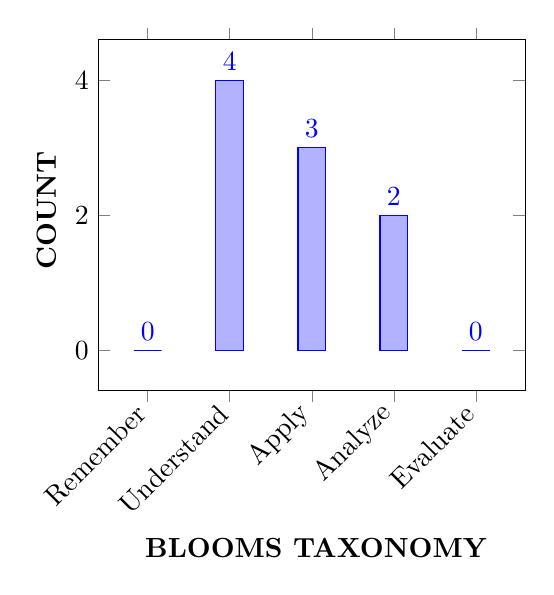
\begin{tikzpicture}  
		\begin{axis}  [
			ybar,
			enlargelimits=0.15,
			legend style={at={(0.5,-0.2)},
				anchor=north,legend columns=-1},
			ylabel={\ \textbf{COUNT} },
			xlabel={\ \textbf{BLOOMS TAXONOMY}},
			symbolic x coords={Remember,Understand,Apply,
				Analyze,Evaluate},
			xtick=data,
			nodes near coords,
			nodes near coords align={vertical},
			x tick label style={rotate=45,anchor=east},
			]
			\addplot coordinates {
				(Remember,0) (Understand,4) (Apply,3)
				(Analyze,2) (Evaluate,0)
			};
		\end{axis}  
	\end{tikzpicture}
\end{center}


\flushleft \textbf{Signature of Course Coordinator}\hspace{8cm} \textbf{HOD, AE}\\\textbf{Mr. K Arun Kumar, Assistant Professor}\\

\end{document}
} 